\section{System Model}
\subsection {Specification Language}

\begin{figure}
    \centering
    \begin{subfigure}[b]{0.3\textwidth}
        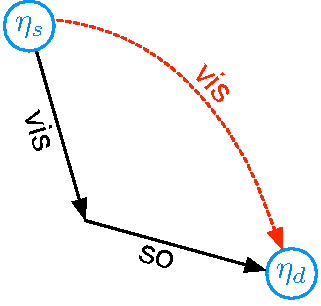
\includegraphics[width=0.66\textwidth]{../Figures/MR.pdf}
        \caption{Monotonic Read (MR)}
        \label{fig:MR}
    \end{subfigure} 
    \hspace{10 mm}
    \begin{subfigure}[b]{0.3\textwidth}
        \centering
        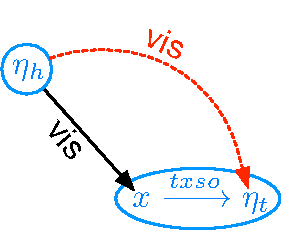
\includegraphics[width=0.66\textwidth]{../Figures/MAV.pdf}
        \caption{Monotonic Atomic View (MAV)}
        \label{fig:MAV}
    \end{subfigure}
    \\ \hrulefill \\
    \caption{Representation of Contracts}\label{fig:contracts}
\end{figure}


Users in our system are offered with a contract language to specify
their application-level consistency requirements.  Developers must
separately define a  contract for each of their application
operations, since the overall correctness of the program does not
require the same level of consistency for all the operations.  The
constructing blocks of contracts are the relations over the set of
effects. Relations $vis(a,b)$ and $so(a,b)$ are defined to relate
effects $a$ and $b$, respectively if $b$ was visible to the operation
that generated $a$ and if they are the result of two operations
submitted by the same session, respecting their submission time. 


Contracts are basically logical formulae that specify the possible sets of effects that are allowed to be visible to an operation. For example, the Monotonic Read (MR) session guarantee, requires all the effects that are visible to an operation, to also be visible to the later operations in the same session. Figure \ref {fig:MR} shows how this can be succinctly defined as a contract using the relations over the effects. This contract simply states that all effects $\eta_h$ that satisfy the relation ($vis^{-1} (so^{-1})$) to an effect $\eta_t$, must also be visible to $\eta_t$. 

%The figure containing the definition of the contract language
\begin{figure}[h]
	\centering
	\begin{minipage}{.75\textwidth}
		$\eta_h,\eta_t, x \in$ EffVar  \hspace {35.5 mm} $Head    ::=    \eta_h | x \xrightarrow{txso} \eta_h | \eta_h \xrightarrow{txso} x$ \\
		$R \in $ Relation ::= $vis | so | R \cup R $ \hspace{20 mm}
		$Tail ::= \eta_t | x \xrightarrow{txso} \eta_t $ \\
		$C \in $ Clause ::= $[R] | R^*$ \hspace{30 mm}		
		$\pi \in$ Prop ::= $(H \xrightarrow{C} T) | \pi \vee \pi$ \\
		$\psi \in$ Contract ::= $ \pi \Rightarrow vis (\eta_h,\eta_t)$ \\
	\end{minipage}
	\\
	\hrulefill
	\caption{The Contract Language}
	\label{fig:ctrt}
\end{figure}

All contracts that can be written in our language, are basically consisted of three parts:
\begin{enumerate}
  \item Head and tail of the contract (e.g. the blue circles in Figure \ref {fig:MR})
  \item The dashed vis edge, that connects head of the contract to its tail, and should be interpreted as the visibility relation \emph{that must be enforced by the system}. 
  \item The linear array of relations connecting head and tail, which represents the relation between the tail and all the effects that must be visible to it.  
\end{enumerate}

Using $vis$ and $so$ relations, users can write a broad set of contracts including all session guarantees from (Terry et. al). In order to allow them to specify even broader set of possible scenarios, we add the notion of transactions to the programs and introduce a new relation $txso$, that relates effects which are related by $so$, and are also in the same transaction. For example, figure \ref{fig:MAV} represents the Monotonic Atomic View (MAV) guarantee, with a tail consisting of $x \xrightarrow {txso} \eta_t$. Note that when the heads or tails are consisted of two effects $x$ and $\eta_{h}$ (or $\eta_{t}$), we implicitly agree to read the dashed $vis$ edge as if it is connected to $\eta_{h}$ (or $\eta_{t}$), and the linear array of relations as if it is connected to the variable $x$.

We structurally limit the use of the $txso$ relation only at the head or the tail of contracts. Figure \ref{fig:ctrt} presents the formal definition of our contract language, that also includes the extended version of the heads and tails of contracts; variables Head and Tail are defined to be either a single effect, or two effects related by $txso$ relation. Note that the dashed $vis$ edge does not require to be explicitly introduced, since it is uniquely defined by its two ends, $\eta_h$ and $\eta_t$.

% The figure containing well known contracts written in our language
\begin{figure}[h]
	\centering
	\begin{minipage}{.88\textwidth}
		{\bf Read My Write (RMW): } \hspace {12 mm}
		$ (\eta_h \xrightarrow{so} \eta_t) \Rightarrow vis (\eta_h,\eta_t) $ \\
		
		{\bf Monotonic Reads (MR): } \hspace {12 mm}
		$ (\eta_h \xrightarrow{vis;so} \eta_t) \Rightarrow vis (\eta_h,\eta_t) $ \\
		
		{\bf Monotonic Writes (MW): } 	\hspace {10 mm}
		$ (\eta_h \xrightarrow{so;vis} \eta_t) \Rightarrow vis (\eta_h,\eta_t) $ \\
		
		{\bf Writes Follow Reads (WFR): } \hspace {5 mm} 	
		$ (\eta_h \xrightarrow{vis;vis} \eta_t) \vee  (\eta_h \xrightarrow{vis;so;vis} \eta_t)  \Rightarrow vis (\eta_h,\eta_t)  $ \\
		
		{\bf Read Committed (RC): } \hspace {14 mm} 		
		$  ((\eta_h \xrightarrow{txso} x)\xrightarrow{vis} \eta_t) \vee 
		((x \xrightarrow{txso} \eta_h)\xrightarrow{vis} \eta_t)  \Rightarrow vis (\eta_h,\eta_t) $ \\
		
		{\bf Monotonic Atomic View (MAV): } 	
		$ (\eta_h \xrightarrow{vis} (x \xrightarrow{txso}  \eta_t))  \Rightarrow vis (\eta_h,\eta_t) $ \\

	\end{minipage}
	\\
	\hrulefill
	\caption{Well-known guarantees specified in our contract language}
	\label{fig:ctrt-examples}
\end{figure}

